\chapter{Performed tests}\label{ch:tests}

We have tested the application in all of its functions. In particular, all the
on-graph queries have been tested multiple times.

\section{User Recommendations}

The user must fill the form shown in \figref{fig:userform} in the application to
perform this query.

\begin{figure}[htb]
	\centering
	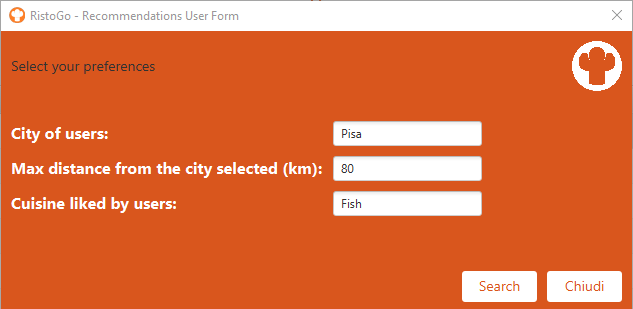
\includegraphics[width=0.8\textwidth]{userform}
	\caption{User Recommendations Application Form.}\label{fig:userform}
\end{figure}

In this test, the query should find users who are not followed by the current
user (``simone''), who live in Pisa or live 80 kilometers away from Pisa, who
likes a Fish cuisine. The resulting users should be sorted by distance from
Pisa.

\figref{fig:subgraph} shows the registered users who like Fish cuisine and the
cities in which they live.

\begin{figure}[htb]%TODO
	\centering
	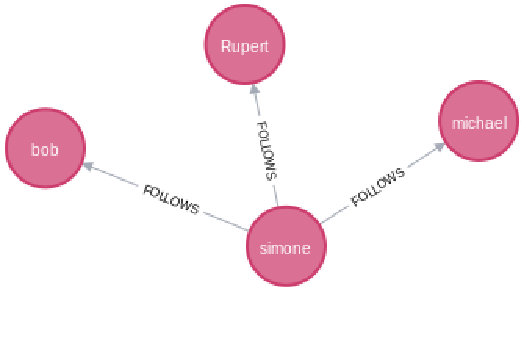
\includegraphics[width=0.8\textwidth]{usersfollowed}
	\caption{Users who like Fish and their cities.}\label{fig:usersfollowed}
\end{figure}

\figref{fig:usersfollowed} shows the users followed by the current user (named
``simone'').

\begin{figure}[htb]%TODO
	\centering
	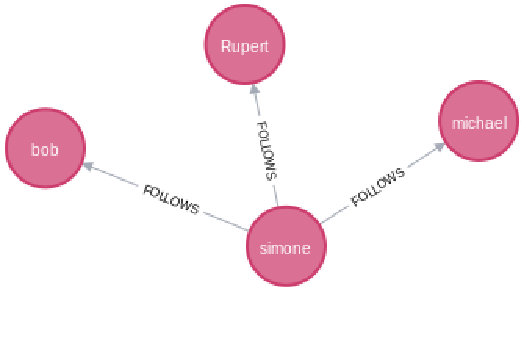
\includegraphics[width=0.8\textwidth]{usersfollowed}
	\caption{Users followed by simone.}\label{fig:usersfollowed}
\end{figure}

So, as you can see from the table, the application returns the correct result as
it shows ``frank'' and ``heidi'' users who are the users who like the Fish
cuisine and who live within a radius of 80 kilometers from Pisa. Note that in
the table, as expected, they are sorted by distance from Pisa.

\begin{figure}[htb]
	\centering
	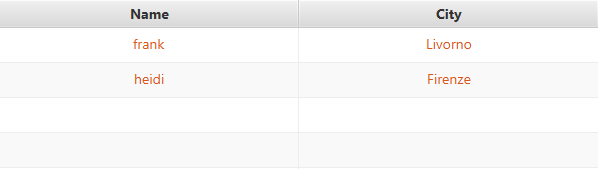
\includegraphics[width=1\textwidth]{tableuserform}
	\caption{Recommended users by the application.}\label{fig:tableuserform}
\end{figure}

\section{Restaurant Recommendations}

We have tested the recommendation on restaurants, here we are providing an
example of the correctness of our results.

Let's suppose to have the following situation, looking at the User ``carol'' we
have the follower/following network in figure

%Aggiungere test_recommend_res1.svg

Now, suppose that carol want to find a restaurant that SERVES Pizza with a Price
ranking of Luxury or lower, at most 80 km distant from Livorno.

\begin{figure}[H]
	\centering
	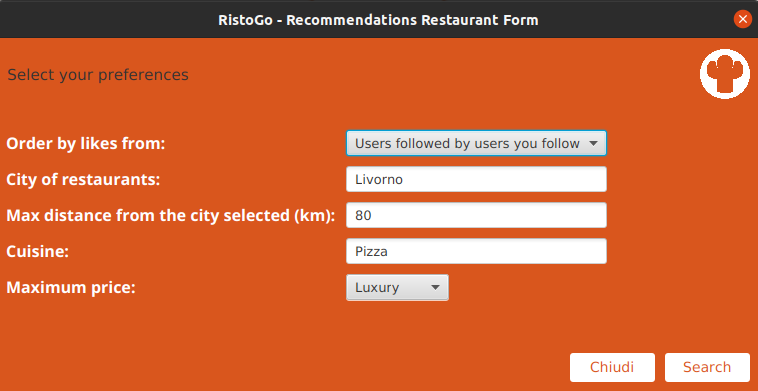
\includegraphics[width=1\textwidth]{test_recommend_filter}
	\caption{Restaurant Recommendations Form.}\label{fig:resrecform}
\end{figure}

In the system we have the following Restaurants which serves Pizza.

%Aggiungere test_recommend_res2.svg

Now the system will suggest to carol the restaurants which serves pizza ordered
by the number of likes of friends and friends of friends and excluding the
restaurants she already likes or owns.

The result provided by the application is the following:

\begin{figure}[H]
	\centering
	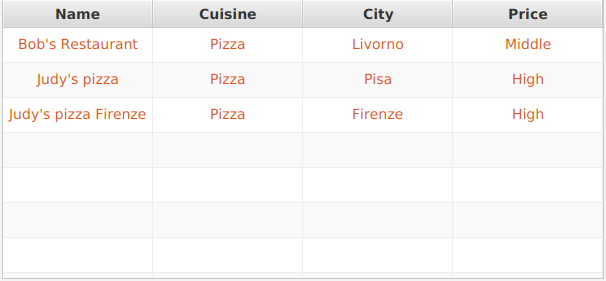
\includegraphics[width=1\textwidth]{test_recommend_result}
	\caption{Restaurant Recommendations Form.}\label{fig:resrecform}
\end{figure}

We can then check in the database that result is correct, in fact looking at the
database we have the situation shown in the graph. In figure are shown only the
relationships from friends or friends of friends of carol with the restaurants
which serves pizza.  Counting the LIKES relationship we can see that effectively
Bob's Restaurant and Judy's Pizza have 3 likes each other, instead Judy's Pizza
Florence has only two likes, thus is shown after.

%Aggiungere test_recommend_res3.svg

Here we can see the results in json:

\begin{verbatim}
    [
  {
    "r": {
"identity": 35,
"labels": [
        "Restaurant"
      ],
"properties": {
"name": "Bob's Restaurant",
"description": "Pizza <3",
"price": "MIDDLE"
      }
    },
    "likes": 3
  },
  {
    "r": {
"identity": 48,
"labels": [
        "Restaurant"
      ],
"properties": {
"name": "Judy's pizza",
"description": "The best pizzas of the world!",
"price": "HIGH"
      }
    },
    "likes": 3
  },
  {
    "r": {
"identity": 49,
"labels": [
        "Restaurant"
      ],
"properties": {
"name": "Judy's pizza Firenze",
"description": "The best pizzas of the world!",
"price": "HIGH"
      }
    },
    "likes": 2
  }
]
\end{verbatim}
